\chapter{Methodology}
\label{cha:methodology}
This section encompasses the methodology employed throughout this thesis. Following an initial exploration of the relevant literature, as discussed in the preceding chapter (see chapter \ref{cha:literature_review}), we outlined our experimentation's blueprint. %The methodology starts with a brief description of the newly defined task of personal narrative elicitation and he new dataset containing personal narratives. Then it branches into two parallel workflows, one dedicated to large language models and ther to crowdsourcing. 
This section includes a definition of the new task of \emph{personal narrative elicitation}, followed by the curation of a new corpus designed for this task. This corpus is composed of narratives for which elicitations were crowdsourced. Then, these human-sourced elicitations are used as reference points against elicitations sourced by prompting LLMs.
% \forgin{itemize}
%     \item The methodology for crowdsourcing encompassed:
%         \begin{itemize}
%             \item \textbf{Guidelines design}: Drafting guidelines tailored for the crowdsourcing component of the study. Those were iteratively reviewed until satisfactory.
%             \item \textbf{User Interface (UI) Design for Crowdsourcing}: Creation of a user-friendly interface incorporating the guidelines previously drafted, ensuring a seamless user experience.
%             \item \textbf{Data collection}: Engaging human crowd workers to participate in the data collection process, collecting responses to our narrative prompts.
%             \item \textbf{Data analysis}: A comprehensive data analysis on the participants' elicitations was conducted.
% convey empathetic     \item Concurrently, for LLMs, the methodology comprised the following key steps:
%         \begin{itemize}
%             \item \textbf{Large Lamodel'se Models selection}: Careful selection of the LLMs that would be subjected to the evaluation. This step is composed of various steps:
%             \begin{itemize}
%                 \item \textbf{Initial Italian language comprehension based selection}: First study conducted on the capabilities of various LLMs to understand the Italian language.
%                 \item \textbf{Story Close Test}: Successive study on the abilities of different LLMs to perform the task of \emph{Story Cloze Test}, which is the most similar task to the task of personal narrative elicitation.
%             \end{itemize}
%             \item \textbf{Personal Narrative Elicitation}: Study of the abilities of personal narratives elicitation across different LLMs:
%             \begin{itemize}
%                 \item \textbf{Design and Formulation of Narrative Elicitation Prompts}: Formulation of prompts aimed at eliciting narratives from the chosen LLMs.
%                 \item \textbf{Experiment}: The investigation is run with the selected prompts across the chosen models.
%             \end{itemize}
%             \item \textbf{Data analysis}: Results from LLMs elicitation are analyzed with various metrics.
%         \end{itemize}
% \end{itemize}
%Ultimately, both workflows converge as both the data generated by LLMs and the data that was acquired through crowdsourcing were systematically compared.
This comparison was executed by utilising both automated and human evaluation metrics. This procedure allowed a comprehensive assessment of the performance of LLMs compared to human crowdworkers on the task of personal narrative elicitation. This evaluation is reported in Chapter \ref{cha:evaluation}.
\section{Eliciting Continuations of Personal Narratives}
We define the task of \emph{eliciting continuations of personal narratives} as the task of prompting specific questions related to a given personal narrative, with the goal of continuing the current narrative, exploring events or topics mentioned in it. Personal narratives are a compelling form of storytelling, representing the recollections of events or connected sequences of events in which the narrator has played an active or passive role. Often intimate and reflective, these narratives are expressed in various mediums, from handwritten diaries to digital travelogues, encompassing both speech and text. The power of personal narratives lies in their ability to convey individual experiences, emotions, and perspectives, making them a rich source of insight into the human condition \cite{noauthor-undated-sy, doi:10.1080/1361332032000044567, Bailey2002-fw} in particular mental health \cite{coadapt}. % CONNECT WITH TEO impictyl SOMEHOW
It is possible to elicit personal narratives through the interview technique, allowing researchers to gather in-depth information on the individual's perspective, beliefs, and lived experiences. It can help researchers understand how people construct and interpret their personal narratives and the meanings they attribute to various events and experiences; for instance, in psychology, elicitation techniques may be employed to improve communication and aid problem-solving. However, eliciting narratives is not trivial, as it requires active listening from the interviewer, with precise questions on topics of the narrative that convey to the narrator an active interest in the narration \cite{Anderson2016-jq}. These questions should also not move the conversation away from the narrator or prompt the narrator to start a new narrative.

In particular, using LLMs for eliciting continuations of personal narratives has some critical requirements for their abilities. For one, it requires LLMs to understand the concept of a conversation between two people, with the LLMs acting as the interviewer. Furthermore, LLMs are also required to understand correctly the events described in the narrative, posing questions on relevant topics mentioned in the narrative or related topics without significantly altering the flow of the narration. Moreover, these narratives may not always use correct grammar or syntax, they may lack a clear and fluent description of the events, and it is up to the interviewer, in this case the LLMs, to understand and piece together the information. Lastly, the questions should be empathetic for narratives of a sorrowful nature, which requires an understanding of empathy and the ability to convey empathetic responses.

We found some existing challenges for LLMs may be helpful, such as \emph{HelloSwag} \cite{HellaSwag}, which tests the ability of a model to understand common sense, and \emph{story cloze test} \cite{mostafazadeh2016corpus}, where a model is tasked to predict the ending of a short story. This story consists of a five-sentence story, of which the model is given as input initial four, and it is tasked to predict the fifth final ending sentence. This last sentence is related to the initial sentences by common sense reasoning. These two tasks can be used as guidance to help address some of the issues with LLMs in the task of eliciting continuations of personal narratives. However, those do not completely solve all our challenges.

In particular, understanding and conveying empathy might be the most challenging, as we found that human crowdworkers also experienced similar issues. For this reason, the dataset presented in this thesis is focused on narratives related to mental health, as it is a topic that is more likely to require empathetic responses, and it also contains specific information regarding the emotion conveyed by certain functional units. In future works, we plan on fine-tuning LLMs on this dataset, with a particular focus on those functional units, to improve the ability of LLMs to convey empathetic responses.

% . It is a task that very closely resembles the Story Close Test \cite{mostafazadeh2016corpus}, but it has a few key differences. In particular:
% \begin{itemize}
%     \item  Eliciting a narrative implies the comprehension of two people in the narration, with one person as the narrator and the other as the listener. Compare this to the story cloze test there is only one story without other roles.
%     \item  Eliciting requires a correct understanding of the context to propose appropriate topics that are both relevant and natural.
%     \item Eliciting requires understanding of concepts such as empathy, as the narrative may be of a sorrowful or joyful nature and it is required to show empathy to the narrator.
%     \item Narratives may not always use correct language syntax and grammar.
%     \item Narratives may be incoherent and/or not follow a clear order of events. It is up to the listener to piece together these inconsistencies and come to an understanding of the topic to elicit correctly.
% \end{itemize}
% Compared to simply asking questions, there are a few caveats that were found in a pilot test during the crowdsourcing process:
% \begin{itemize}
%     \item Questions should be inherent to topics and/or elements present in the narrative.
%     \item A proper elicitation should not involve questions on hypothetical scenarios or personal opinions because they start a new narrative.
%     \item Elicitations should not move the focus away from the narrator.
%     \item Elicitations cannot be suggestions, because suggestions do not elicit.
% \end{itemize}

\section{Dataset}
Given the absence of a pre-existing dataset tailored for the task of eliciting continuations of personal narratives, the decision was made to perform a data collection to produce a new dataset. This dataset was augmented from the CoAdapt dataset, as documented in \cite{coadapt}. The CoAdapt dataset was initially collected within the framework of a psychological study focusing on mental health. The inception of the dataset involved soliciting users' responses daily, with a fixed set of questions presented to them. Data for \emph{Emotion Carriers} and \emph{Valence} was collected. Emotion Carriers are people, objects or events that indirectly convey emotions \cite{tammewarannotation}, while Valence represents the level of sadness or joy, measured on a scale from -2 to +2, of functional units of the narrative \cite{Ong2021-yt,roccabruna-etal-2022-multi}. 

\begin{table}[!htbp]
\centering
\caption{An example of original data and the respective emotion carriers and valences. On the first column, the division in questions, and on the second, the respective textual answers. Emotion carriers, reported in the third column convey narrators’ emotions in the text. The last column reports the values of valence which represents in a range from -2 to +2 the level of sadness or joy of the respective highlighted sections.}
\label{tab:dataset-coadapt-example-ec-valence}
    \centering
    \begin{tabularx}{\linewidth}{ l | X | p{2cm} | c}
        \toprule
        \multicolumn{4}{c}{ \thead{Coadapt Original Data}}\\
        \midrule
        \thead{Question} & \thead{Answer} & \thead{Emotion \\ Carrier} & \thead{Valence}\\
        \midrule
        % \arrayrulecolor{lightgray}
        initial note &  \highLight[highlightgreen]{Serenità coi fiori}  &  \multicolumn{1}{c|}{$\sim$} & +1\\[1em]
        % \midrule
        cbt response a & Domenica nel mio giardino & \multicolumn{1}{c|}{$\sim$}& 0 \\[1em]
        % \midrule
        cbt response b &  \highLight[highlightgreen]{Sarebbe bello poter avere un profumo simile a quello delle viole o dell' iris} &  poter avere, un profumo & +1\\[1em]
        % \midrule
        cbt response c & Occupandomi dei miei fiori \highLight[highlightgreen]{ho sentito una sensazione piacevole data dal profumo delle viole e dal sole che leggero accarezzava la pelle. Ho provato Felicità} nelle parti del corpo: Testa sensazione di inebriamento. & ho sentito, profumo, vuole, sole, accarezzava & +1 \\[1em]
        % \arrayrulecolor{black}
        \bottomrule
    \end{tabularx}
\end{table}

An example is shown in Table \ref{tab:dataset-coadapt-example-ec-valence}
\begin{table}
\centering
\caption{Table reporting an example of original data and revision that was applied to it. The original data is composed of answers to a set of 4 questions, which is not structured in a narrative format. Therefore manual review was applied in order to get a coherent and fluid narrative.}
\label{tab:dataset-coadapt-example}
    \centering
    % \begin{tabularx}{p{2cm}|p{3cm}|p{5cm}|p{5cm}}
    \begin{tabularx}{\linewidth}{ l | p{10cm} | X }
        \toprule
        \multicolumn{2}{c|}{ \thead{Coadapt Original Data}} & \thead{Revised Narrative}\\
        \midrule
        \thead{Question} & \thead{Data} & \multirow{5}{3.5cm}{Domenica nel mio giardino, occupandomi dei miei fiori ho sentito una sensazione piacevole data dal profumo delle viole e dal sole che leggero accarezzava la pelle. Sarebbe bello poter avere un profumo simile a quello delle viole o dell' iris. }\\
        \cmidrule{1-2}
        % \arrayrulecolor{lightgray}
        initial note & Serenità coi fiori &  \\ [1em]
        % \cmidrule{1-2}
        cbt response a & Domenica nel mio giardino \\ [1em]
        % \cmidrule{1-2}
        cbt response b & Sarebbe bello poter avere un profumo simile a quello delle viole o dell' iris \\ [2em]
        % \cmidrule{1-2}
        cbt response c & Occupandomi dei miei fiori ho sentito una sensazione piacevole data dal profumo delle viole e dal sole che leggero accarezzava la pelle. Ho provato Felicità nelle parti del corpo: Testa sensazione di inebriamento.\\[4em]
        % \arrayrulecolor{black}
        \bottomrule

    \end{tabularx}
\end{table}

The dataset in question was collected in the Italian language, with the active participation of native Italian speakers as data contributors. Nonetheless, carefully considering the dataset curation process becomes important, given the intrinsic variability of human responses to such questions. There were instances when the user did not answer some of the questions or answered to multiple questions simultaneously. As shown in the previous Table, it is impossible to simply concatenate the texts together to obtain a fluent narrative. Doing so would create incoherent narratives with no clear flow and missing linguistic conjunctions. This is due to the fact that the questions are not designed to elicit a continuation of the narrative but rather to elicit a response to those specific questions related to mental health.
For this reason, the dataset was manually reviewed and refined to ensure a coherent narrative flow. This process involved the addition of conjunctions and linguistic modifications, ensuring a seamless and cohesive narrative flow. Additionally, the dataset underwent an anonymisation procedure, which entailed the removal of any references to specific locations or individuals, replacing instead with randomly selected alternatives. Narratives deemed excessively brief were removed, while longer narratives were strategically divided into multiple narratives.
% \begin{table}
\centering
\caption{Table reporting an example of revised data and the respective splits that were done on it.}
\label{tab:dataset-coadapt-example-split}
    \centering
    \begin{tabularx}{\linewidth}{X|X|X }
        \toprule
        \thead{Revised Narrative \\Part 1} & \thead{Revised Narrative \\Part 2}  & \thead{Revised Narrative \\Complete}\\
        \midrule
        Stamattina mia mamma mi ha mandato un messaggio perché era preoccupata per il mio papà. & Stamattina mia mamma mi ha mandato un messaggio perché era preoccupata per il mio papà. Andava da solo a farsi esami del sangue e aveva paura che potesse avere un incidente con la macchina perché ultimamente guida poco e non è più abituato. & Stamattina mia mamma mi ha mandato un messaggio perché era preoccupata per il mio papà. Andava da solo a farsi esami del sangue e aveva paura che potesse avere un incidente con la macchina perché ultimamente guida poco e non è più abituato. Ero a casa con i miei figli che si stavano preparando per andare a scuola. Ho pensato che lui sta invecchiando ed è in difficoltà ma anche che lei fa fatica ad accettarlo e gli trasmette ancora più ansia oltre che ad accumulare lei altrettanta. \\
        \bottomrule

    \end{tabularx}
\end{table}

% In light of this issue, a thorough manual review and refinement process was done to imbue coherence and narrative fluency into the dataset. This review process encompassed the addition of conjunctions and linguistic modifications, ensuring a seamless and cohesive narrative flow. Additionally, the dataset underwent an anonymization procedure, which entailed the removal of any references to specific locations or individuals, replacing instead with randomly selected alternatives. Narratives deemed excessively brief were removed, while longer narratives were strategically divided into multiple narratives, as exemplified in Table \ref{tab:dataset-coadapt-example-split}.

The result was a dataset tailored for the specific task of eliciting continuations of personal narratives. Notably, this dataset comprises a total of 476 narratives, thoughtfully divided into two subsets: 419 narratives for the training set and 57 narratives for the test set.
% \begin{table}[ht]
\centering
\caption{Table reporting a short and a long example of narratives.}
\label{tab:dataset-coadapt-example-short-long}
    \centering
        \begin{tabularx}{\linewidth}{ p{3cm} |X }
        \toprule
        \multicolumn{2}{c}{\thead{Revised Narratives}} \\
        \midrule
        \textbf{Short narrative example} & Dopo oltre 7 mesi stasera ho potuto rivedere la zia di 94 anni. Ho pensato al mio primo bambolotto che mi ha regalato proprio lei. \\[2em]
        \textbf{Long narrative example} & Stamattina mia mamma mi ha mandato un messaggio perché era preoccupata per il mio papà. Andava da solo a farsi esami del sangue e aveva paura che potesse avere un incidente con la macchina perché ultimamente guida poco e non è più abituato. Ero a casa con i miei figli che si stavano preparando per andare a scuola. Ho pensato che lui sta invecchiando ed è in difficoltà ma anche che lei fa fatica ad accettarlo e gli trasmette ancora più ansia oltre che ad accumulare lei altrettanta. \\
        \bottomrule
    \end{tabularx}
\end{table}
\begin{table}[!htbp]
\centering
\caption{Report of some statistics computed from narratives present in the dataset. Reported are the number of narratives, average narrative length and standard deviation in number of tokens and the number of unique words for the complete dataset, as well as the splits of train and test sets. Tokenization was done through Spacy}
\label{tab:dataset-coadapt-statistics}
    \centering  
    \begin{tabular}{l|rrr}
    % \begin{tabularx}{\linewidth}{  X | X | X | X }
        \toprule
        \multicolumn{4}{c}{\thead{Statistics of the narratives}}\\
        \midrule
        \thead{Statistic} & \thead{Train Set} & \thead{Test Set} & \thead{Overall Set}\\
        \midrule
        Number of narratives& 419 & 57 & 476 \\[1em]
        Average narrative length & 50.4 & 44.4  & 49.5 \\
        Standard deviation on narrative length & 38.9 & 31.3 & 37.9 \\[1em]
        Number of unique words & 3225 & 629 & 3378 \\
        \bottomrule

    \end{tabular}
\end{table}

An analysis of tokens was conducted using the Spacy tokeniser to gain further insights into the linguistic properties of the dataset. Punctuation marks, stop words, and numerical digits were excluded from this analysis, revealing the presence of 3,376 unique tokens within the dataset. Each narrative prompt spans 49.5 tokens on average, with a notably high standard deviation of 37.8. These statistics can be found in Table \ref{tab:dataset-coadapt-statistics}. 

\begin{figure}[!htbp]
    \centering
    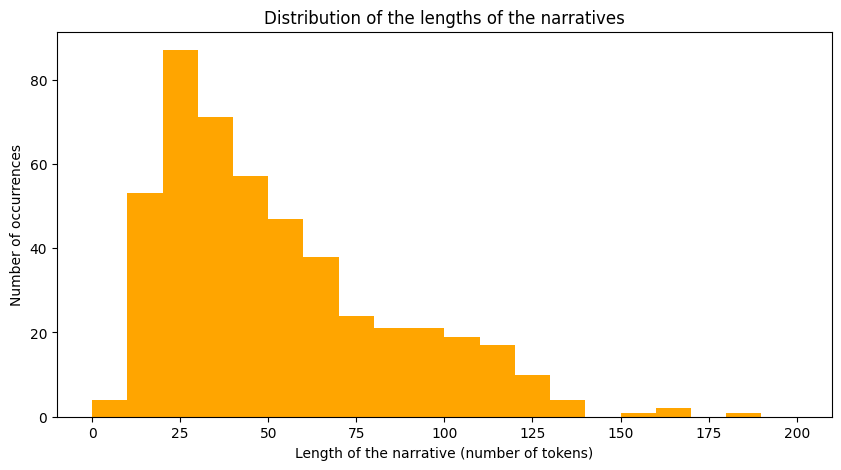
\includegraphics[width=1\linewidth]{assets//imgs/dataset-length-distribution.png}
    \caption{Barchart of the length distribution. There are a few narratives that are very short, while others are very long, but the majority of the narratives are between 30 and 70 tokens.}
    \label{fig:dataset-length-distruibution}
\end{figure}
The token count in some prompts is as low as 5, while others extend well beyond 200 tokens, attesting to the diversity of the dataset in terms of textual length, reported in Figure \ref{fig:dataset-length-distruibution}. % Example is shown in Table \ref{tab:dataset-coadapt-example-short-long}

\begin{figure}[!htbp]
    \centering
    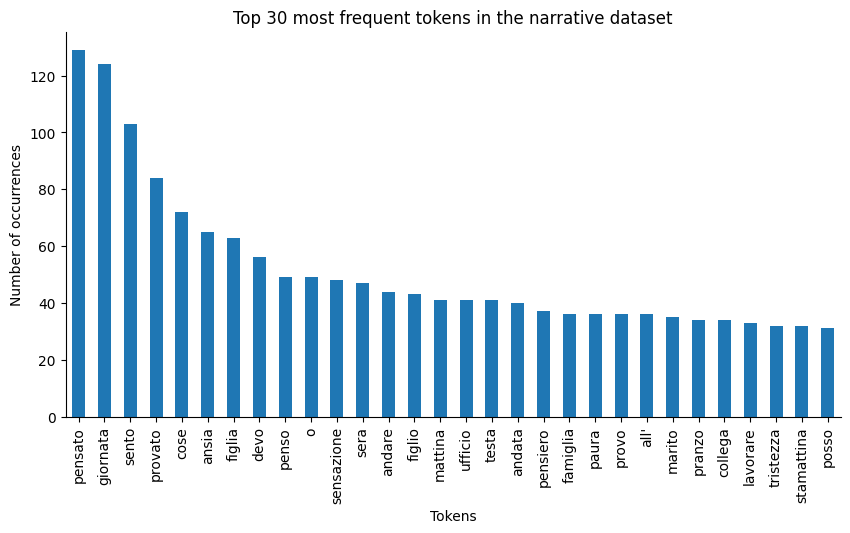
\includegraphics[width=1\linewidth]{assets//imgs/dataset-top-30-prompt.png}
    \caption{Barchart of the top 30 most frequent tokens in the dataset. Notice how the most frequent tokens are related to anxiety, day, feelings, work, and family. This aligns with the thematic focus on mental health of the dataset.}
    \label{fig:dataset-top-30-prompt}
\end{figure}

Besides those statistics, a bar chart of the top most frequent 30 tokens is illustrated in Figure \ref{fig:dataset-top-30-prompt}. As depicted in the figure, some of the most frequently occurring tokens align seamlessly with the inherent thematic focus on mental health and domains of mental health, work, and family of the dataset.
% \emph{"giornata"}, \emph{"ansia"},  \emph{"dispiace"},  \emph{"figlia"},  \emph{"figlio"}, and  \emph{"lavoro"}. These tokens 

